

\section{Yago}
\begin{frame}
\frametitle{YAGO Yet Another Great Ontology}

\includegraphics[scale=0.25]{img/yago_logo_small.png}
\begin{itemize}
\item YAGO (2008) YAGO2s (2012)
\item developed at Max Planck Institute for Computer Science
\item more than 10 million entities
\item more than 120 million facts
\end{itemize}
%YAGO in its newest Version YAGO2s is a very big knowledgebase developed at the Max Planck Institute for Computer Science. In 2012, YAGO2s had knowledge of more than 10 million entities and contained more than 120 million facts about these entities.
\end{frame}

\begin{frame}
\frametitle{Extraction from:}

\includegraphics[scale=0.31]{img/yago-figure2.png}
%These are exclusively extracted from: Wikipedia, WordNet, GeoNames, WordNet Domains (,which augments WordNet with domain labels) and the Universal WordNet (which is the multilingual approach on WordNet).\\
\end{frame}

\begin{frame}
\frametitle{Extracts from Wikipedia:}
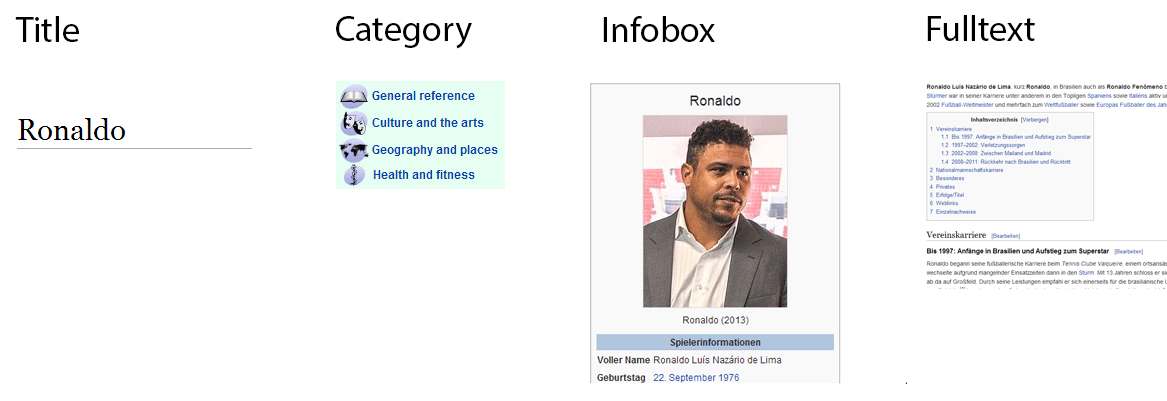
\includegraphics[scale=0.25]{img/yago-figure3.png}
%Now we have already one big knowledge-base which is extractin from Wikipedia, DBpedia, why do we need YAGO. Well, for one YAGO extracts the infoboxes, categories and fulltext, whereas DBPedia only takes the infoboxes.
\end{frame}

\begin{frame}[fragile]
\frametitle{Relations:}
\begin{itemize}
\item YAGO:\\
about predefined relations with domain and range:\\
\begin{lstlisting}[frame=single]
:hasSon rdfs:domain :Person;
            rdfs:range  :Man.
\end{lstlisting}
adds temporal and spatial dimension to many entities/relations
\item DBpedia:\\
uses words from infoboxes\\
$\rightarrow$ length, length-in-km, length-km
\end{itemize}
%Then YAGO has about 100 manually predefined relations with domains and ranges, while DBPedia uses the words it finds in the infoboxes. As a drawback the same relation may appear with different names.
\end{frame}

\begin{frame}
\frametitle{Precision and costs}
\begin{itemize}
\item YAGO:
\begin{itemize}
\item manually evaluated that 95% triplets are correct
\item extractions process lasts 3 days
\item over 12 researcher
\end{itemize}
\end{itemize}
%All this make YAGO a very precise database. A manual evaluation confirmed that 95\% of the triplets extracted by YAGO are correct. But this comes at the price of speed and maintenance. Because YAGO draws from few but very different sources, the extraction, reconciliation, deduplication, verification of constraints, etc. takes several days to run. Plus more than a dozen researches, who need to work directly or indirectly on YAGO.\\
\end{frame}

\begin{frame}
\frametitle{Why YAGO?}
\begin{tabular}{l|c|r}
& YAGO & DBpedia\\
\hline 
extracts: & title, category, infobox, fulltext & infobox\\
relations: & predefined (domain, range) & taken from infobox\\
precision: & very good & not that good \\
costs: & very high & not that high

% Here we see again a direct comparision between YAGO and DBpedia
\end{tabular}
\end{frame}

\begin{frame}
\frametitle{Extraction-process and Sources}
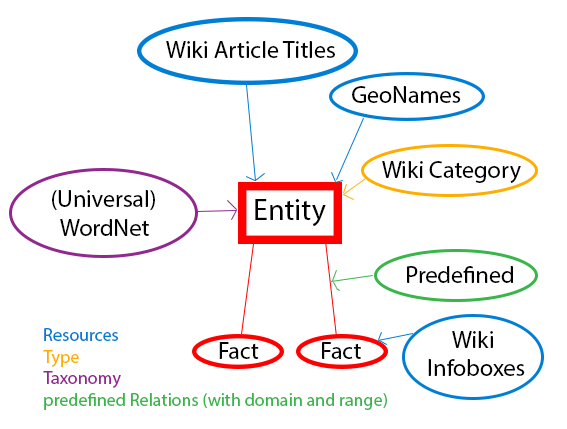
\includegraphics[scale=0.35]{img/yago-ex1.png}
%The extraction of the original YAGO looks like this. The titles of the Wikipedia articles contribute the entities. The wikipedia-categories are analyzed to derive the entities type. Then the infoboxes are extracted to get facts about the entity, which are stored in predefined relations. WordNet and Universal WordNet deliver the taxonomic backboneand then GeoNames is used to merge additional Entities into the ontology.
\end{frame}

\begin{frame}
\frametitle{YAGO2s}
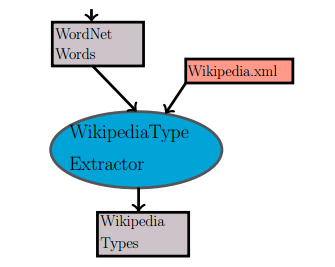
\includegraphics[scale=0.7]{img/yago_figure.PNG}
%YAGO2s introduced a transparent and modular architecture. Main ingredients are themes and extractors.\\
%A theme, represented by these rectangles, is a collection of facts, such as all facts derived from WordNet, or facts concerning people. These facts are completely RDF compliant and stored in turtle format with additional fact identifiers to integrate time and space information. \\
%Then we have extractors, these ellipses. Extractors have a number themes as input and a number of themes as output. Such as an extractor for deduplication which takes a number of themes as input and puts a deduplicated theme out. Then there are also Extractors which can take external data sources as input, represented as these smaller rectangles. For example the Wikipedia Category Extractor, which takes Wikipedias XML-dump as input and produces a theme with facts extracted from Wikipedia-categories.\\
\end{frame}

\begin{frame}
\frametitle{Visualization}
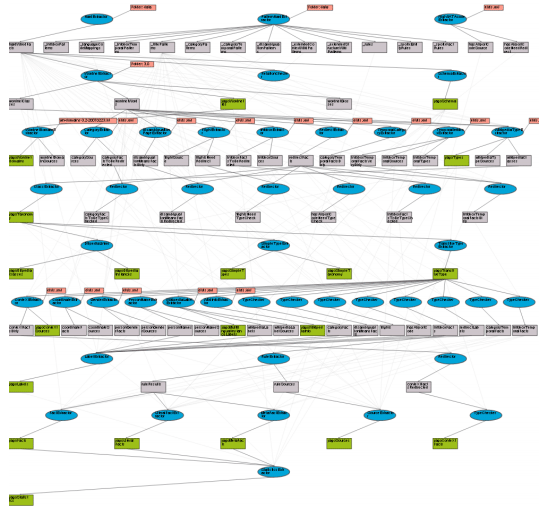
\includegraphics[scale=0.32]{img/yago_visual.png}\\
http://resources.mpi-inf.mpg.de/yago-naga/yago/www2013demo/yago\_demo\_static/
%This is a visualization of all these extractors and themes as a dependency graph. It also integrates the scheduling constraints of YAGO. Some extractors have to be executed in a certain order and some can be executed in parallel. The lines show which extractor rpodues which theme and which theme is used by which extractor. We can see four main types of extractors: Wikipedia extractors which are exclusively concerned with Wikipedia-sources, GeoNames which harvest and map entities from GeoNames, External extractors which extract from (Universal) WordNet and WordNet domains and Theme Extractors which exclusively take Themes as input, such as the deduplicator or a constraints checker. Some extractors, for example the Type Checker, are instantiated multiple time, so that the overall amount of extractors in this visualization rises from 30 unique to 42 extractors.\\
%Another interesting extractor would be the WordNet domains extractor which enriches the entities with domains such as "law" or "music". This enable you to ask for all entities which are related to "music" for example.
\end{frame}

\begin{frame}
\frametitle{Demo Ontology Browser}
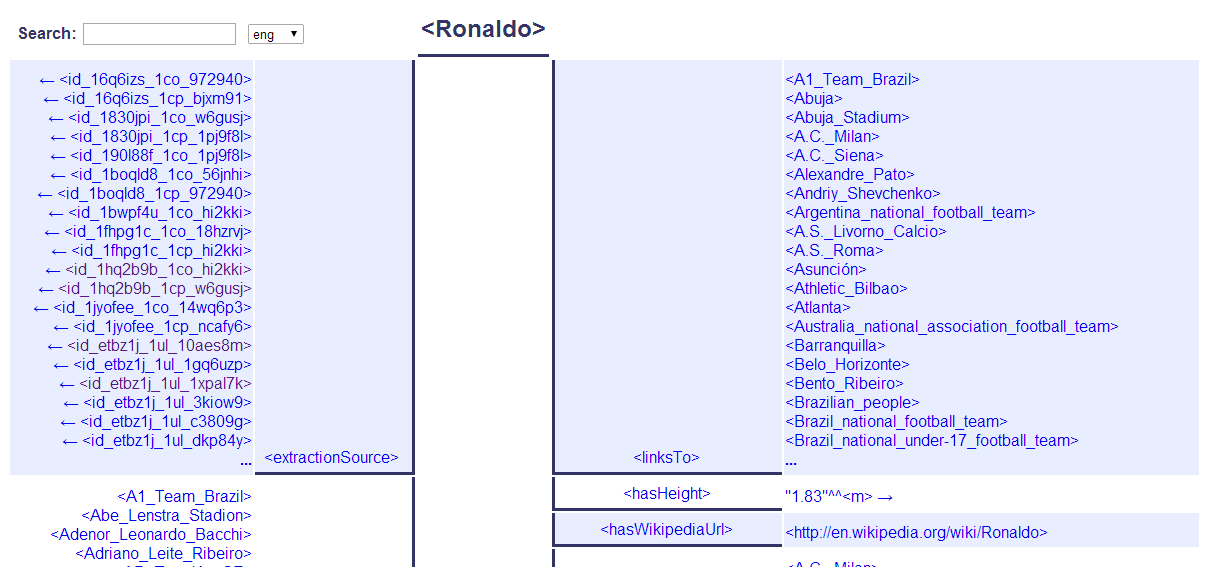
\includegraphics[scale=0.2]{img/yago-obr.png}\\
https://gate.d5.mpi-inf.mpg.de/webyagospotlx/Browser
\end{frame}

\begin{frame}
\frametitle{Demo spotlx}
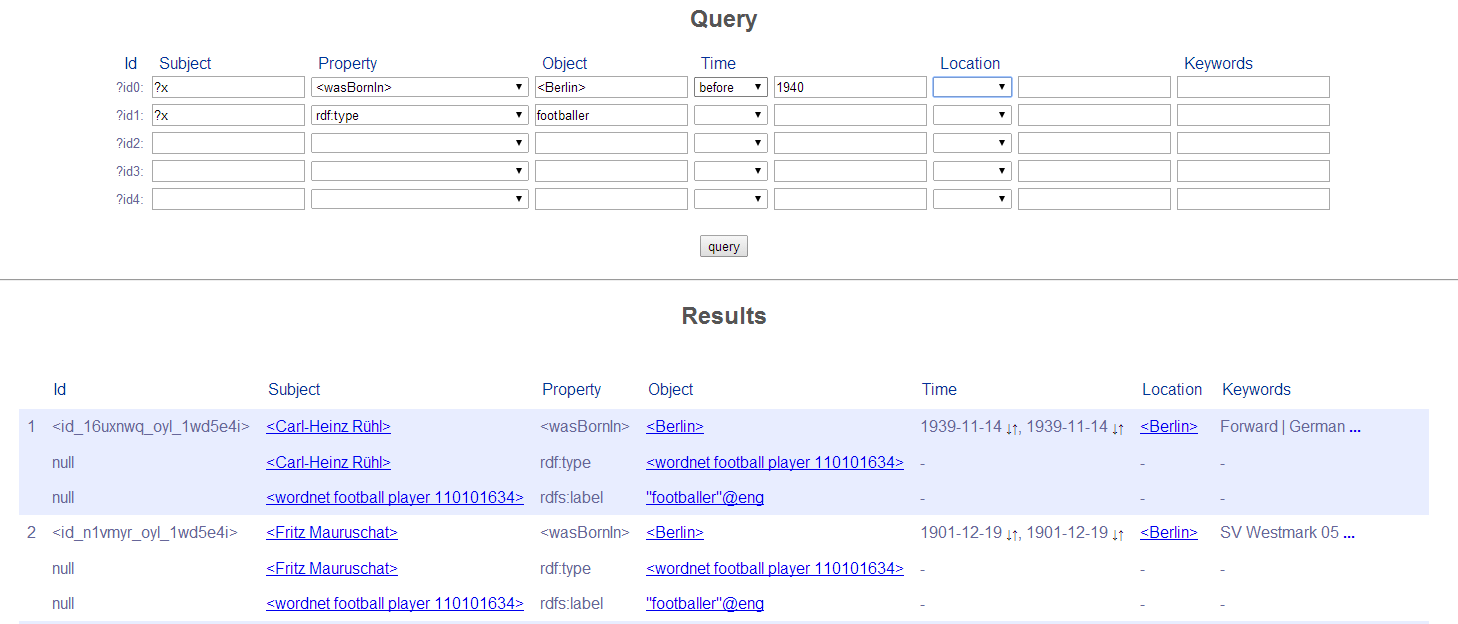
\includegraphics[scale=0.2]{img/yago-spotnx.png}\\
https://gate.d5.mpi-inf.mpg.de/webyagospotlx/WebInterface
\end{frame}
